\documentclass{article}
\usepackage{graphicx}
\usepackage[utf8]{inputenc}
\usepackage{setspace}
\usepackage{float}
\usepackage[margin=1in]{geometry}
\usepackage{booktabs}
\usepackage{hyperref}
\usepackage{footnote}
\usepackage{float}

\title{African Music Network Dataset Project}
\author{Mark Lekina Rorat}
\date{June 5, 2023}

\begin{document}

\maketitle

\begin{center}
    \texttt{\url{https://github.com/marklekina/african_music_dataset_project/}}
\end{center}

\doublespacing\section{Introduction}

This report presents a new network dataset of African music artists and track
data. We demonstrate how we collected artist and track metadata using the
Spotify API, and artist nationality data through web scraping of the African
musicians Wikipedia page. We also conducted some investigations on the dataset,
namely the correlation between the proportion of collaborations and artist
nationality/genre, the evolution of collaboration patterns over time, and the
relationship between collaboration and artist popularity. Through statistical
analyses, we provide insights into the African music industry and potential
opportunities for fostering collaborations and promoting African artists on a
global scale. First, we describe our dataset through the data collection and
preprocessing workflow. Next, we present the results of our analyses coupled
with a summary of our findings. Finally, we conclude with the limitations of
our work and suggestions for future research.

\section{Dataset overview}
\subsection{Data sources}

To build our network dataset, we utilized these two data sources:

\begin{itemize}
    \item \textit{Spotify} API\footnote{\url{https://developer.spotify.com/}}: This API provides extensive artist and track data spanning various genres and time periods. We used the API to gather valuable information such as track popularity, artist follower counts, and other relevant metadata.

    \item \textit{Wikipedia}\footnote{\url{https://en.wikipedia.org/wiki/List_of_African_musicians}}: Despite its breadth, the Spotify API does not include artist nationality data. For this reason, we scraped the Wikipedia page listing African musicians to collect nationality information for the artists.
\end{itemize}

\subsection{Data collection}

During the data collection phase, we utilized two scripts to gather the
necessary information:

\begin{itemize}
    \item \texttt{fetch\_spotify\_data}: This script was responsible for querying the Spotify API to retrieve artist and track data. Using the \texttt{spotifyr} library, we made API calls and obtained JSON responses. The script then parsed these responses using the \texttt{jsonlite} library, converting them into structured data frames for further analysis.
    \item \texttt{scrape\_nationality\_data}: This script focused on crawling artist Wikipedia pages to extract information about their nationalities. Using the \texttt{rvest} library, we performed web scraping to collect the desired data. The script compiled the nationality information into a central dataset, which would later be merged with the Spotify data.
\end{itemize}

\begin{figure}[H]
    \centering
    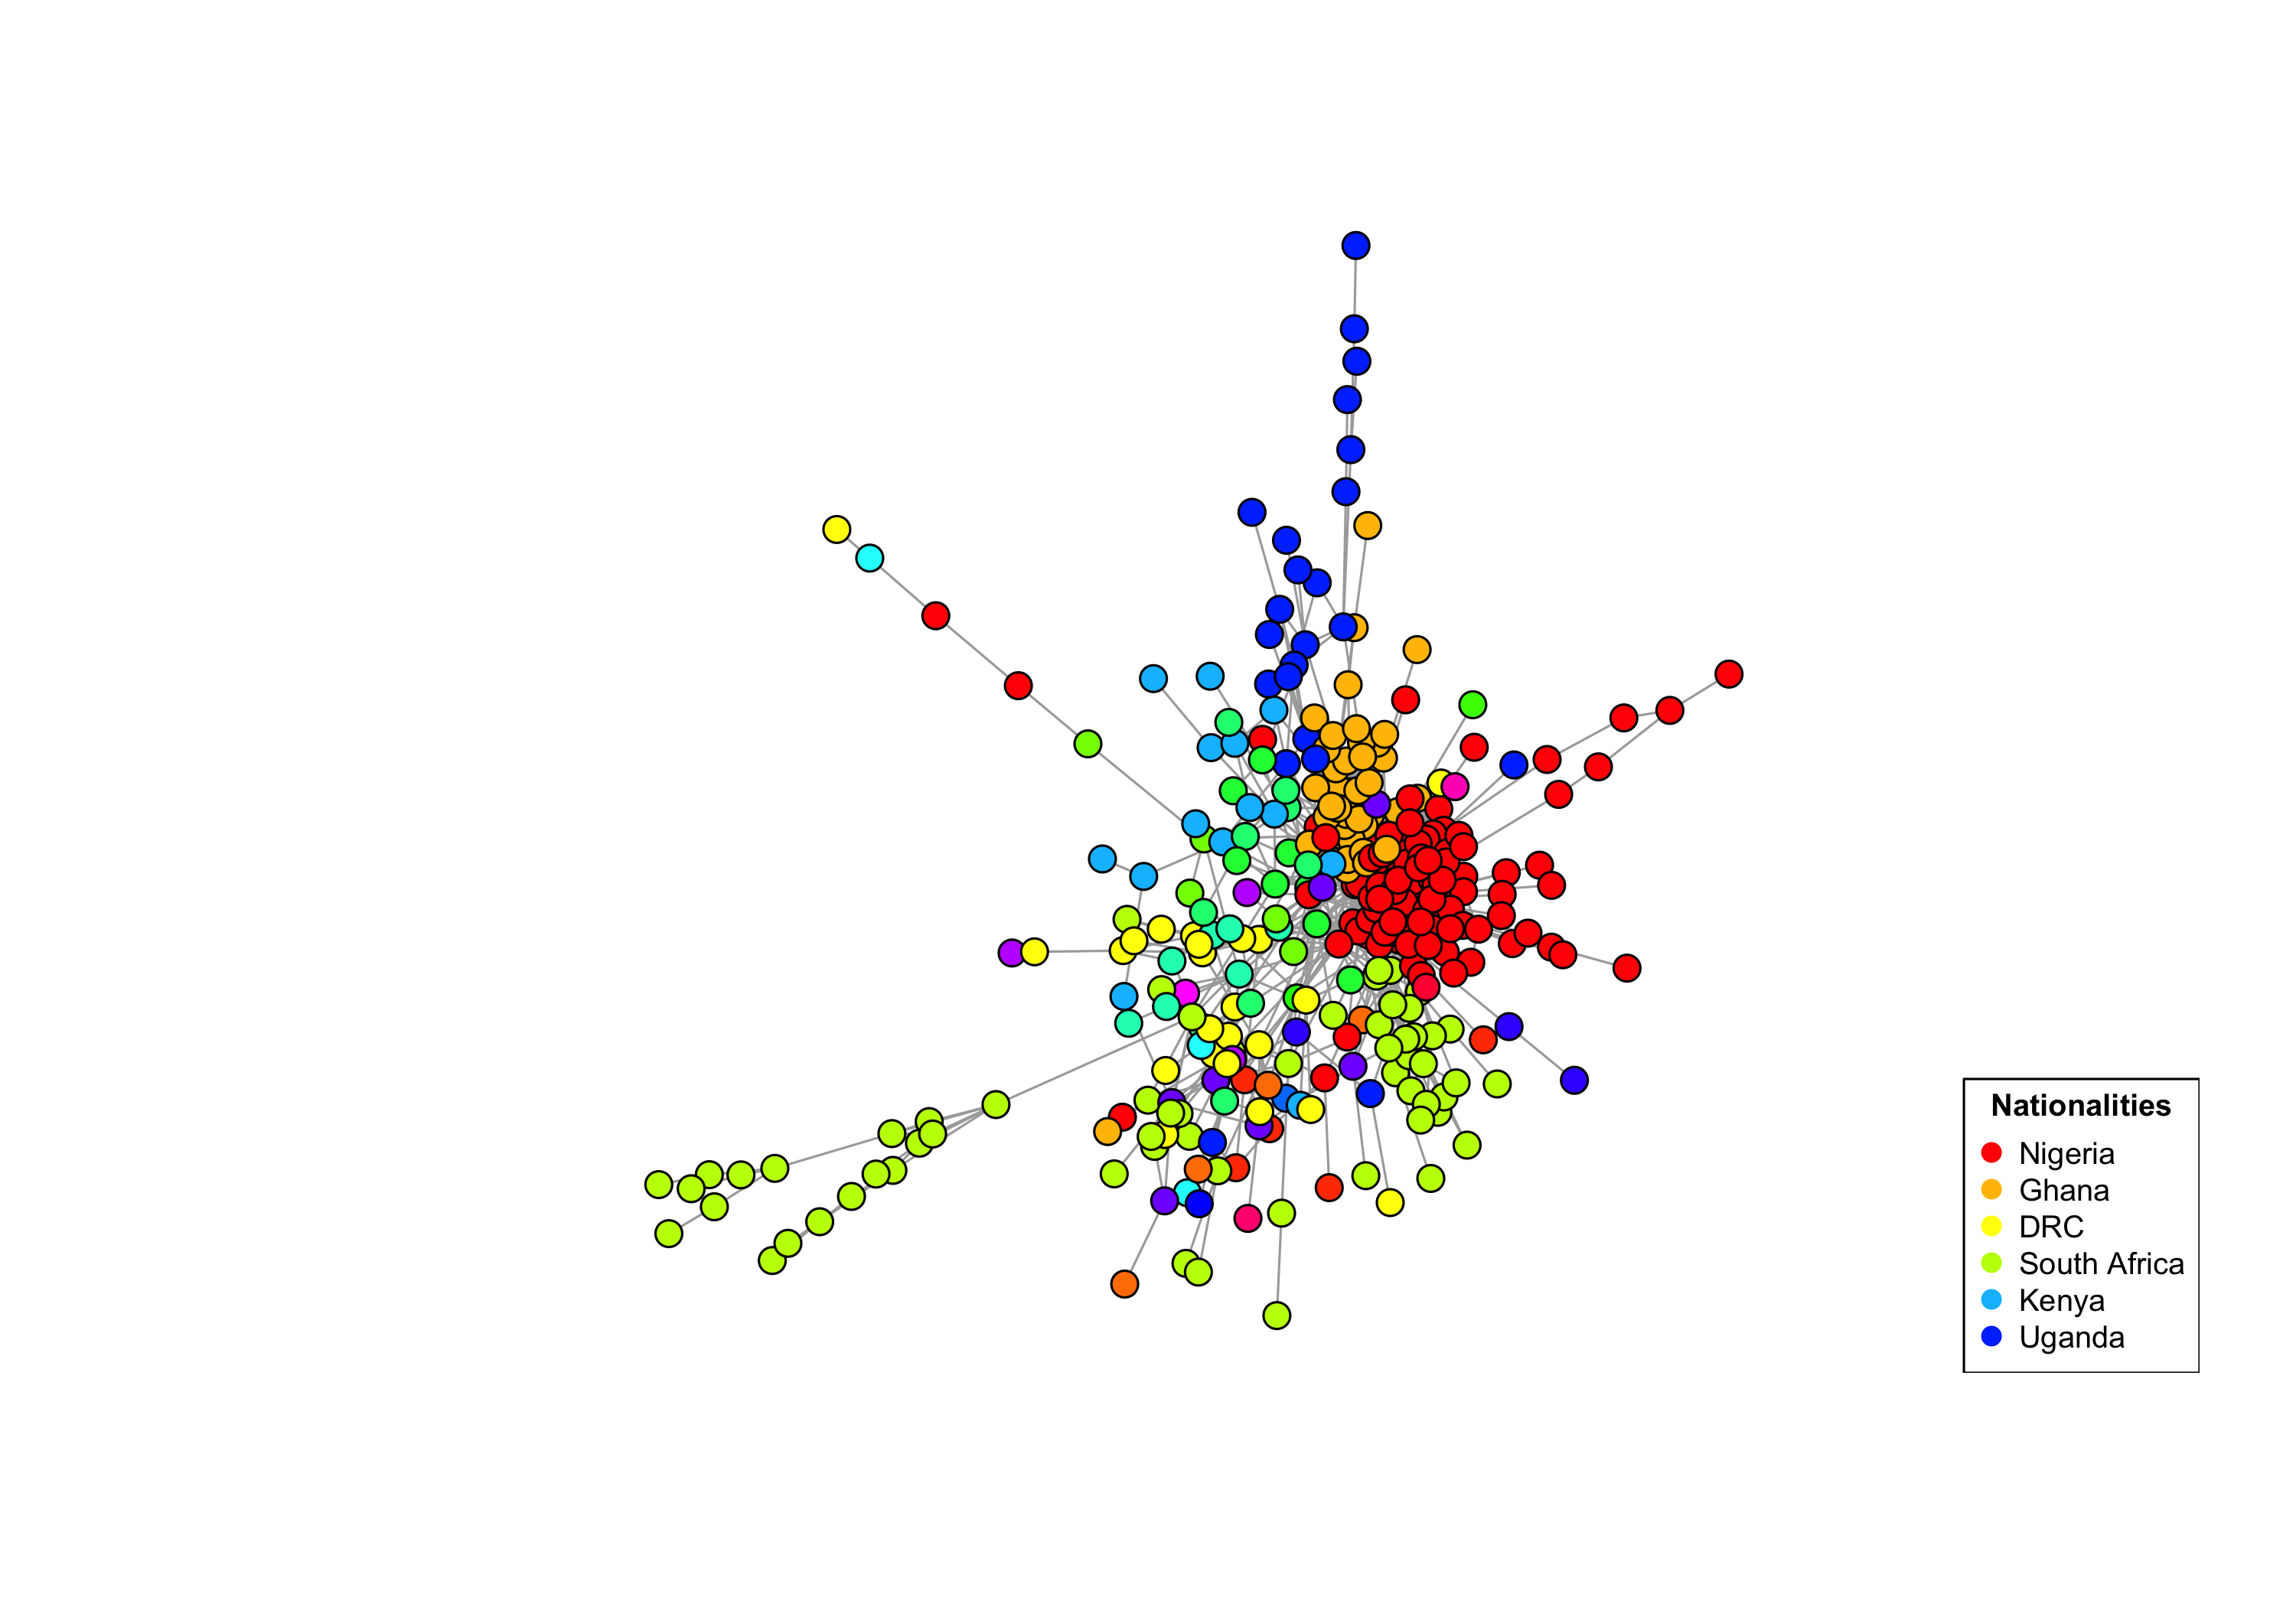
\includegraphics[width=\textwidth]{../data/figures/african_artist_network_countries.png}
    \caption{Network of African Artists by Country}\label{fig:network_countries}
\end{figure}

\subsection{Data collection workflow}

The data collection workflow involved several steps to gather the required
information for our analysis. Here is an overview of the process:

\begin{enumerate}
    \item Starting with the base URL for African musicians on Wikipedia, we fetched the
          HTML content from webpages containing lists of artist names grouped by country.
    \item We performed web scraping on the base webpage to extract the artist names and
          country information. These details were stored in a data frame.
    \item For countries that had links to webpages with artist names instead of directly
          listing them, we navigated to those pages and scraped the artist names into the
          data frame.
    \item Using the artist names collected from Wikipedia, we utilized the Spotify API's
          search endpoint to fetch artist objects for each name. We only considered exact
          matches to ensure relevance.
    \item To supplement our list of artists, we retrieved the related artists for each
          artist using the Spotify API's related artists endpoint.
    \item After gathering all the necessary artist objects, we parsed the artist metadata
          from the JSON responses and stored it in a data frame.
    \item To collect track data, which was required for aggregating collaboration
          information, we employed two approaches:
          \begin{itemize}
              \item First, we obtained the top tracks for each artist using the appropriate API
                    endpoint.
              \item Second, we searched for track objects by artist name. We then subsetted the
                    results to include only tracks where the artist ID matched the ID provided in
                    the track's list of artists.
          \end{itemize}
    \item Once we had collected all the track JSON objects, we parsed the track metadata
          into a separate data frame.
\end{enumerate}

\subsection{Data preprocessing workflow}

After data collection, we did some data preprocessing to prepare the collected
data for analysis. For this part, we used the \texttt{preprocessing\_analysis}
script to perform the data preprocessing tasks and some preliminary analysis.
Here is an overview of the process:

\begin{enumerate}
    \item The first step was merging the artist Spotify data with the nationality data
          collected from Wikipedia.
    \item Next, we addressed the issue of duplicate tracks in the track data. Since each
          track has a unique ID, we couldn't deduplicate based on ID alone. Instead, we
          compared the list of artists performing the track and the raw version of the
          track's name after removing whitespace and matching cases. If both matched, we
          selected the track with the highest popularity and dropped the duplicates.
          Typically, the most popular track corresponds to the original album release,
          while the duplicates may be compilation releases or versions not by the artist.
    \item The next step involved building the network adjacency matrix from the track and
          artist data. We first subsetted the data to include only tracks with more than
          one artist. Each artist in these tracks is considered a \textit{node} in the
          network, and an \textit{edge} represents a collaboration between two artists.
          The \textit{weight} of each edge is the number of collaborations between the
          artists in the track dataset.
    \item We pruned the network to include only edges between known African artists. This
          is because some of our analysis requires nationality data, which is not
          available for each node. From this subset, we induced a subgraph from the
          largest connected component of the graph. The final result was a graph with 342
          \textit{nodes} and 1111 \textit{edges}, spanning 23 \textit{countries}. Figure\
          \ref{fig:network_countries} visualizes the network. Each node is colored to
          match the artist’s nationality, and the colors for the countries with the
          highest number of nodes in the network are indicated in the legend.
\end{enumerate}

\subsection{Strengths of the dataset}

One of the strengths of this dataset is that it represents the first
comprehensive effort to aggregate African music data into a coherent and
publicly available dataset. It brings together information from multiple
sources, including the Spotify API and Wikipedia, to provide a comprehensive
view of African music artists and their music. The dataset incorporates
nationality data from Wikipedia, which enriches the artist and track metadata
obtained from Spotify. This additional information allows for a more
comprehensive understanding of the artists and their cultural backgrounds.

Another strength of the dataset is its balanced representation of artists from
different African countries. Efforts were made to ensure that the dataset is
not biased towards artists from countries with more popular music scenes. The
Spotify API was queried for data on artists from each African country listed on
the Wikipedia page, ensuring a diverse representation of artists. Furthermore,
the transparency of the dataset is a notable strength. The code used for data
collection, preprocessing, and analysis is publicly available, allowing for
reproducibility and modification. This openness provides opportunities for
researchers to improve the dataset and enhance its quality over time.

\subsection{Weaknesses of the dataset}

One of the main weaknesses of the dataset is the challenge of obtaining
comprehensive and accurate data on artist nationalities. The availability of
extensive and high-quality nationality data for artists is crucial for
conducting meaningful analyses. However, this information is often incomplete
or inaccurate. One challenge is that the Wikipedia web pages on African artists
cannot possibly list all artists from each specific country. As a result, it is
impossible to fetch artist metadata for a significant majority of artists from
a particular country. This limitation restricts the dataset's coverage and may
result in an incomplete representation of artists from certain countries.

Additionally, some Wikipedia pages may incorrectly list the nationality of
certain artists. This is particularly common for artists who have gained global
popularity but are not necessarily of African nationality, but have African
ancestral roots. Detecting and correcting these inaccuracies at scale is a
difficult task. As a result, relying on nationality data to diversify the
dataset and conduct further analysis becomes challenging, as low-quality
nationality data can undermine the accuracy of the findings.

To address this issue, the dataset had to be subsetted to include only artists
whose nationalities are Wikipedia-verified. This necessary step in ensuring
data quality and accuracy results in a significant loss of data that could have
otherwise been valuable for analysis. Consequently, the final network dataset
includes only 23 nationalities, despite starting data preprocesssing with
artists from over 45 different nationalities. Overall, the limitations in
obtaining comprehensive and accurate artist nationality data pose a significant
weakness in the dataset. It highlights the challenges faced in compiling a
comprehensive dataset for African music and the need for further efforts to
improve data quality and coverage.

\section{Analysis and Findings}

The key questions we wanted to investigate for our analysis are the following:

\begin{enumerate}
    \item How does proportion of collaborations vary by country?
    \item Which genres tend to have the highest (or the lowest) proportion of
          collaborations?
    \item How has collaboration between African artists evolved over time?
    \item Is there a correlation between collaboration and the popularity of artists?
\end{enumerate}

\subsection{Preliminary analysis}

We addressed the first three questions through straightforward analysis
methods:

\subsubsection{Collaboration Proportion by Artist Nationality}

\begin{table}[H]
    \centering
    \begin{tabular}[t]{lrr}
        \toprule
        country                          & collaboration\_proportion & collaboration\_count \\
        \midrule
        Swaziland                        & 0.7435897                 & 29                   \\
        South Sudan                      & 0.5671642                 & 38                   \\
        Tanzania                         & 0.4983165                 & 148                  \\
        Benin                            & 0.4285714                 & 30                   \\
        Nigeria                          & 0.3707527                 & 1724                 \\
        Ghana                            & 0.3647235                 & 732                  \\
        Kenya                            & 0.3397933                 & 263                  \\
        Democratic Republic of the Congo & 0.3146269                 & 527                  \\
        Cape Verde                       & 0.2888889                 & 13                   \\
        Mali                             & 0.2820513                 & 165                  \\
        \bottomrule
    \end{tabular}
    \caption{Top 10 countries with the highest proportion of collaborative tracks}\label{tab:top_collab_countries}
\end{table}

To analyze the proportion of collaborations based on artist nationality, we
merged the track data with artist nationality data and calculated the number of
rows (\textit{i.e.}, tracks) where each unique country name appeared for both
singles and collaborations. The collaboration proportion was computed as the
ratio of collaboration count to the total count. The countries with the highest\
and lowest collaboration proportions are presented in Tables\
\ref{tab:top_collab_countries} and\ \ref{tab:top_single_countries}. As
expected, countries with a larger number of artists in the network tended to
have higher collaboration proportions.

\begin{table}[H]
    \centering
    \begin{tabular}[t]{lrr}
        \toprule
        country               & single\_artist\_proportion & single\_artist\_count \\
        \midrule
        Eritrea               & 1.0000000                  & 46                    \\
        Guinea-Bissau         & 0.9772727                  & 43                    \\
        Togo                  & 0.9759036                  & 81                    \\
        Sudan                 & 0.9743590                  & 38                    \\
        Sierra Leone          & 0.9655172                  & 56                    \\
        Gabon                 & 0.9647059                  & 82                    \\
        Botswana              & 0.9245283                  & 49                    \\
        Egypt                 & 0.9184028                  & 529                   \\
        Guinea                & 0.8983051                  & 159                   \\
        Republic of the Congo & 0.8673469                  & 170                   \\
        \bottomrule
    \end{tabular}
    \caption{Top 10 countries with the highest proportion of single-artist tracks}\label{tab:top_single_countries}
\end{table}

\subsubsection{Collaboration Proportion by Artist Genres}

\begin{table}[H]
    \centering
    \begin{tabular}[t]{lrr}
        \toprule
        genre                    & collaboration\_proportion & collaboration\_count \\
        \midrule
        amapiano                 & 1.0000000                 & 13                   \\
        baroque singing          & 1.0000000                 & 10                   \\
        british modern classical & 1.0000000                 & 28                   \\
        early modern classical   & 1.0000000                 & 28                   \\
        impressionism            & 1.0000000                 & 28                   \\
        post-romantic era        & 1.0000000                 & 28                   \\
        sgija                    & 1.0000000                 & 13                   \\
        gqom                     & 0.9729730                 & 36                   \\
        igbo traditional         & 0.9354839                 & 29                   \\
        edm                      & 0.8604651                 & 37                   \\
        \bottomrule
    \end{tabular}
    \caption{Top 10 genres by collaboration proportion}\label{tab:top_collab_genres}
\end{table}

\begin{table}[H]
    \centering
    \begin{tabular}[t]{lrr}
        \toprule
        genre                & single\_artist\_proportion & single\_artist\_count \\
        \midrule
        african gospel       & 1                          & 42                    \\
        black punk           & 1                          & 34                    \\
        botswana traditional & 1                          & 43                    \\
        congolese gospel     & 1                          & 42                    \\
        gospel amapiano      & 1                          & 3                     \\
        microtonal           & 1                          & 39                    \\
        ngoni                & 1                          & 43                    \\
        oromo pop            & 1                          & 9                     \\
        sierra leonean pop   & 1                          & 14                    \\
        south african metal  & 1                          & 17                    \\
        \bottomrule
    \end{tabular}
    \caption{Top 10 genres by single-artist proportion}\label{tab:top_single_genres}
\end{table}

For this analysis, we utilized genre data available in the artist Spotify
metadata. The metadata includes a list of genres commonly associated with an
artist's music. Similar to the nationality analysis, we computed the
collaboration proportions for each genre by merging track data with artist
genre data. The results are shown in Tables\ \ref{tab:top_collab_genres} and\
\ref{tab:top_single_genres}. Our qualitative analysis revealed that non-native
genres, such as classical and impressionism music, tend to feature more
collaborations, while country-specific indigenous music often leans towards
singles.

\subsubsection{Collaboration Over Time}

\begin{figure}[H]
    \centering
    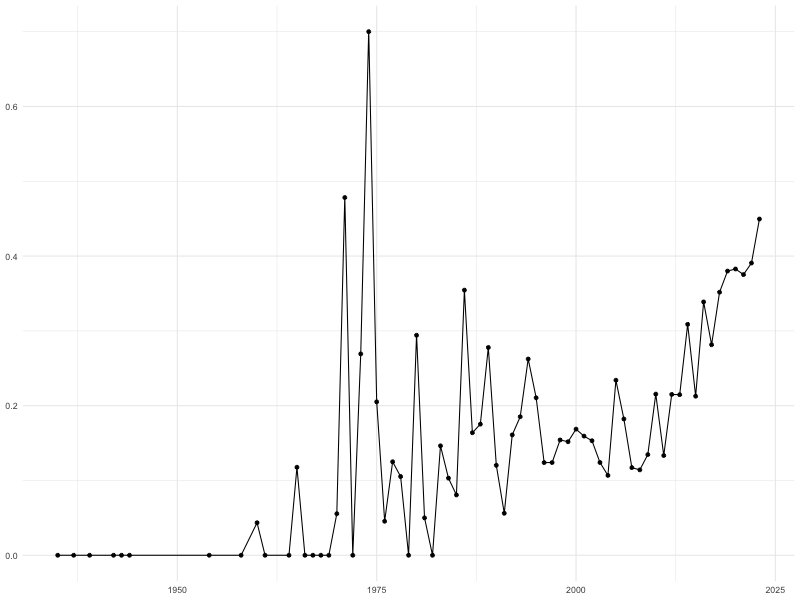
\includegraphics[width=\textwidth]{../data/figures/collaboration_proportions_by_time.png}
    \caption{Proportion of collaborative tracks over time}\label{fig:time_collab}
\end{figure}

To investigate the temporal evolution of collaboration, we grouped the track
data by the release year of albums (extracted from the album's release date in
track metadata) and computed the collaboration proportions. Figure\
\ref{fig:time_collab} presents a plot of collaboration proportions of the
results over time. Although the proportion of collaborations exhibits a peak in
the mid-70s, the overall volume of collaborations tends to increase over time.
However, it is important to note that this observation may be influenced by the
larger presence of recent tracks in the dataset, and further analysis is needed
to draw definitive conclusions.

By conducting these analyses, we aimed to gain insights into the correlation
between artist popularity and artist network centrality measures. These
findings provide a foundation for understanding the dynamics of collaboration
within the African music industry.

\subsection{Network analysis}

\subsubsection{What is the significance of the network’s centrality measures in predicting artist popularity?}

\begin{table}[H]
    \centering
    \begin{tabular}[t]{llrrrr}
        \toprule
        centrality\_measure & term        & estimate     & std.error    & statistic & p.value \\
        \midrule
        betweenness         & (Intercept) & 3.531621e+01 & 0.9489058    & 37.217826 & 0.0e+00 \\
        betweenness         & value       & 4.367100e-03 & 0.0007625    & 5.727709  & 0.0e+00 \\
        closeness           & (Intercept) & 1.821336e+01 & 3.8605889    & 4.717766  & 3.5e-06 \\
        closeness           & value       & 3.008932e+04 & 5786.9529144 & 5.199510  & 3.0e-07 \\
        degree              & (Intercept) & 3.156899e+01 & 1.0988871    & 28.728144 & 0.0e+00 \\
        degree              & value       & 9.578788e-01 & 0.1149585    & 8.332387  & 0.0e+00 \\
        eigenvector         & (Intercept) & 3.554460e+01 & 0.9401270    & 37.808296 & 0.0e+00 \\
        eigenvector         & value       & 4.311637e+01 & 7.8108501    & 5.520061  & 1.0e-07 \\
        page\_rank          & (Intercept) & 2.967162e+01 & 1.3210111    & 22.461298 & 0.0e+00 \\
        page\_rank          & value       & 2.777305e+03 & 355.6898172  & 7.808221  & 0.0e+00 \\
        \bottomrule
    \end{tabular}
    \caption{Linear Regression of Artist Popularity on Individual Centrality Measures}\label{tab:centrality_regression_individual}
\end{table}

In order to examine the relevance of the network's centrality measures in
predicting artist popularity, we calculated various centrality measures for the
network and conducted linear regression analysis. The centrality measures
served as independent variables, while artist popularity was the dependent
variable. The results of the analysis are presented in Table\
\ref{tab:centrality_regression_individual}.

The analysis reveals that higher centrality measures tend to correspond to
higher artist popularity, as indicated by the consistently higher intercept
estimates. The p-values associated with each centrality measure are extremely
close to zero, suggesting a high level of statistical significance for each
measure.

These findings highlight the importance of centrality measures in predicting
artist popularity within the network. Artists who exhibit higher centrality, as
indicated by measures such as betweenness, closeness, degree, eigenvector, and
page rank, are more likely to have a greater level of popularity. The strong
statistical significance of these centrality measures further supports their
relevance in understanding and predicting artist popularity within the network.

\subsubsection{How well do community structures in the network predict artist popularity?}

\begin{table}[H]
    \centering
    \begin{tabular}[t]{lrrrr}
        \toprule
        term        & estimate   & std.error & statistic & p.value \\
        \midrule
        (Intercept) & 45.9821075 & 1.2118217 & 37.94461  & 0       \\
        community   & -0.7030323 & 0.0589465 & -11.92661 & 8.6e-33 \\
        \bottomrule
    \end{tabular}
    \caption{Logistic Regression of Artist Popularity on Community Membership}
\end{table}\label{tab:community_regression}

To assess the predictive power of community structures in the network on artist
popularity, we utilized the \textit{Girvan-Newman algorithm} to detect
communities based on \textit{edge-betweenness centrality}. The resulting
community structures are visually represented in Figure\
\ref{fig:network_communities}.

Since the community membership variable derived from the algorithm is
categorical rather than numerical, we applied \textit{one-hot encoding} and
employed logistic regression to build a model. In this model, artist popularity
served as the dependent variable, while community membership was the
independent variable. The outcomes of the logistic regression analysis are
presented in Table\ \ref{tab:community_regression}.

The results demonstrate that community membership significantly influences an
artist's popularity. The p-values, which are close to zero, indicate a highly
significant relationship between an artist's community membership and their
level of popularity. Figure\ \ref{fig:network_communities} provides a
qualitative examination of the community structures, revealing that while
artist nationality predominantly defines the communities, there are also
instances where communities extend beyond national boundaries in the denser
parts of the network.

Considering the previous findings that centrality measures, including node
betweenness centrality, exhibit a statistically significant relationship with
artist popularity, it follows that community memberships defined by
edge-betweenness centrality also possess a significant association with an
artist's popularity. This emphasizes the importance of community structures in
understanding and predicting artist popularity within the network.

\begin{figure}[H]
    \centering
    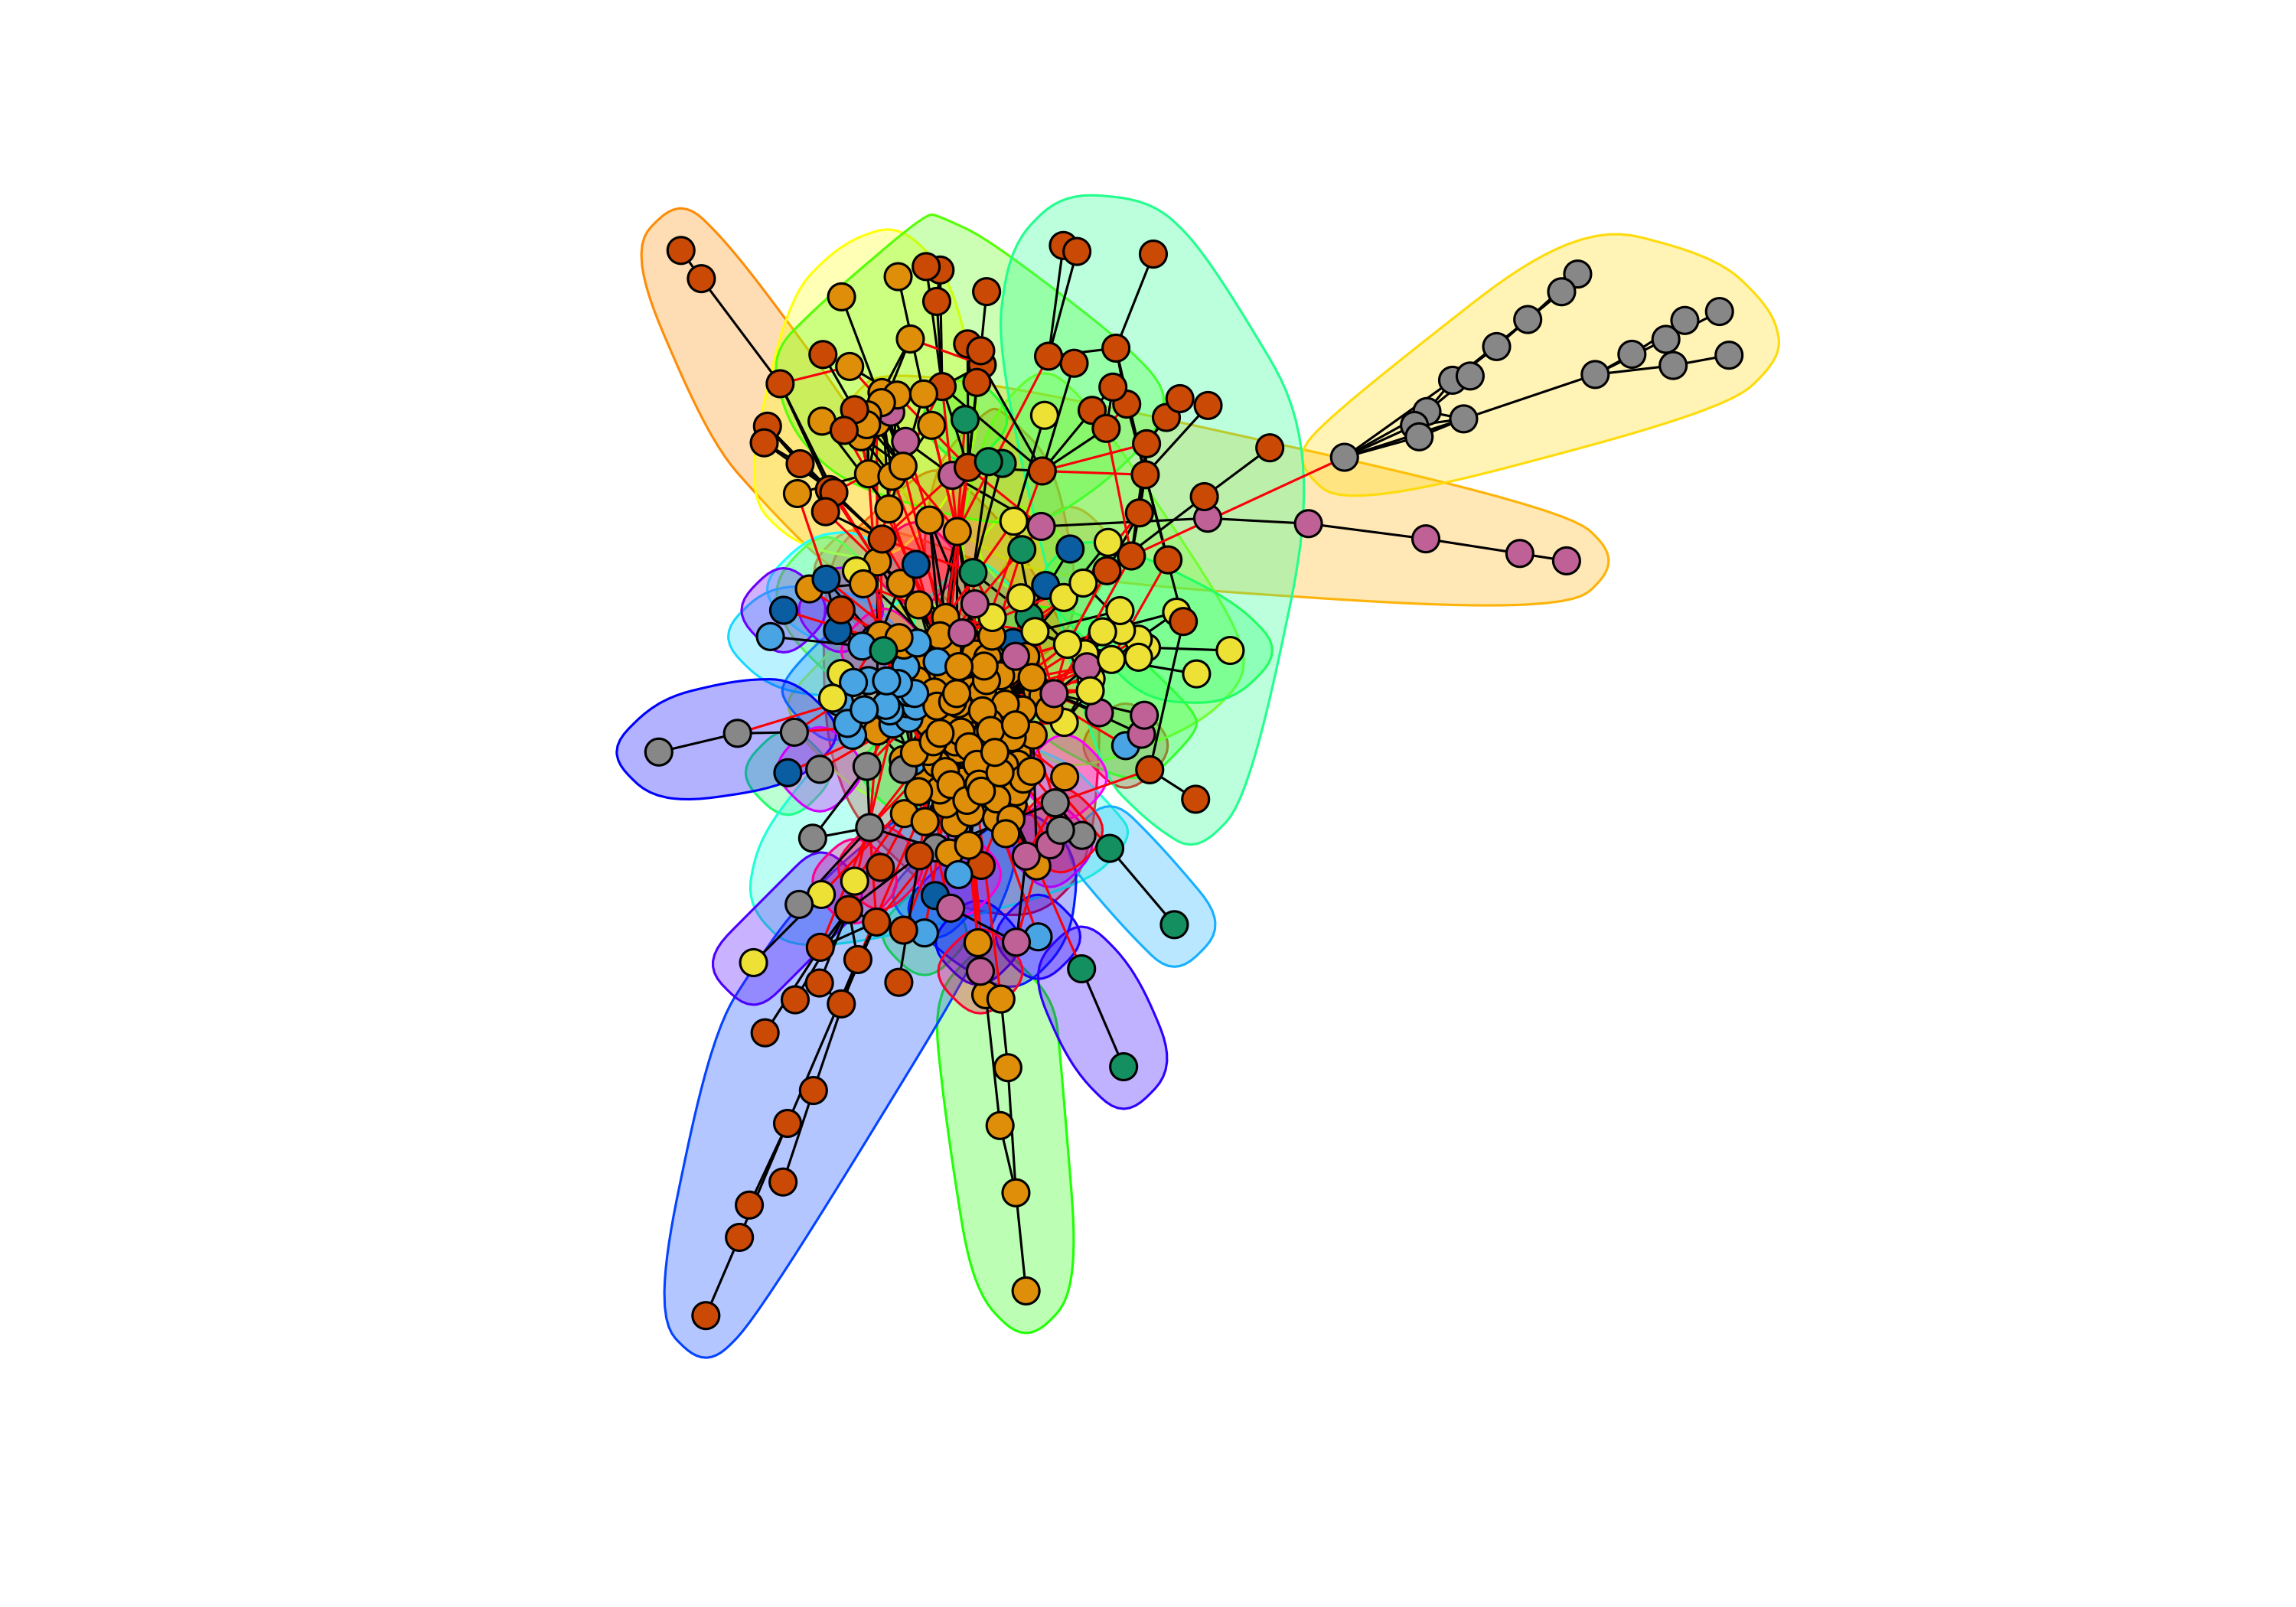
\includegraphics[width=\textwidth]{../data/figures/african_artist_network_communities.png}
    \caption{Network of African Artists by Communities}\label{fig:network_communities}
\end{figure}

\section{Conclusion}

In conclusion, this report has presented a comprehensive analysis of African
music artists and their collaborations using a dataset that combines
information from Spotify and Wikipedia. Through the careful collection and
preprocessing of data, we have been able to explore various aspects of
collaboration within the African music industry and draw meaningful insights.

Our analysis revealed several interesting findings. Firstly, we observed
variations in the proportion of collaborations based on artist nationality and
genre. Non-native genres tended to feature more collaborations, while
country-specific indigenous music often leaned towards singles. This highlights
the diverse nature of African music and the influence of cultural and
genre-specific factors on collaboration patterns.

Additionally, we investigated the evolution of collaboration over time and
observed a general increasing trend in the volume of collaborations. While
collaboration reached its peak in the mid-70s, the presence of recent tracks in
the dataset may have skewed this observation. Nevertheless, this analysis
provides valuable context to understand the historical development of
collaborations within the African music industry.

Furthermore, our study explored the relationship between collaboration and
artist popularity using centrality measures and community structures within the
network. The results indicated that higher centrality measures tend to be
associated with higher artist popularity, suggesting the significance of
network centrality in predicting artist success. Additionally, community
membership, identified through the Girvan-Newman algorithm, emerged as a
significant predictor of artist popularity, highlighting the influence of
community structures on an artist's recognition and reach.

It is important to acknowledge the limitations of our analysis. One key
challenge was the availability and quality of artist nationality data, which
required us to subset the dataset to Wikipedia-verified nationalities,
resulting in a loss of valuable data. Additionally, the dataset may not capture
the entire African music landscape, as it relies on the availability of artist
data on Spotify and Wikipedia.

Nevertheless, this study represents an important step in understanding and
appreciating the vibrant collaborations within the African music industry. The
findings can inform stakeholders in the music industry, policymakers, and
researchers interested in African music by providing valuable insights into the
dynamics of collaboration and its impact on artist success. Moving forward, we
hope to continue expanding and refining the dataset, incorporating data from
additional sources and exploring other dimensions of collaboration, such as
cross-border collaborations and the influence of social and cultural factors.

Overall, this analysis contributes to the growing body of research on African
music and underscores the richness, diversity, and potential of the African
music industry. By embracing collaborations and leveraging the unique cultural
heritage of African music, we can celebrate its global impact and foster its
continued growth and recognition.

\end{document}